% Provenance (never printed): cycle 4 SVT/physique, "La planete Terre,
% l'environnement": the atmosphere, its structure and its layers, pressure
% and altitude, the ozone layer; see sources/book1/PROVENANCE.md. Book 1,
% grade 8, chapter 1.
% Vocabulary guard: owns the layers of the atmosphere (troposphere,
% tropopause, stratosphere, mesosphere, thermosphere), the environmental
% lapse rate and the ozone layer. Air pressure and the barometer are the
% physics books' (recalled), the composition of air and ozone the molecule
% the chemistry books'; "convection cell" is g8.2's and is not used here;
% adiabatic cooling is Book 2's.
\chapter{De atmosfeer}\label{ch:g8:the-atmosphere}

Op een \omterm{def:g4:clouds-rain-snow:weather-station}{weerstation} loopt een meteoroloog vlak voor het afgesproken uur het
grasveld op met een ballon gevuld met waterstof of helium, ongeveer
\qty{1.5}{m} in doorsnee. Daaronder hangen aan een lang touw een kleine
oranje parachute en een instrumentkastje van 60 tot 80 gram: een
\emph{radiosonde}. Ze laat los. De ballon stijgt ongeveer \qty{300}{m} per
minuut, en elke seconde zendt de radiosonde de druk, de temperatuur, de
luchtvochtigheid en haar positie door. Terwijl de ballon stijgt, zwelt hij
op, tot hij 6 tot \qty{8}{m} in doorsnee is en knapt, vaak meer dan
\qty{30}{km} hoog, twee uur na de lancering. Op dezelfde uren van elke dag
speelt hetzelfde tafereel zich af op meer dan 800 stations over de hele
wereld.
% ledger: nws:radiosonde

\begin{omfigure}
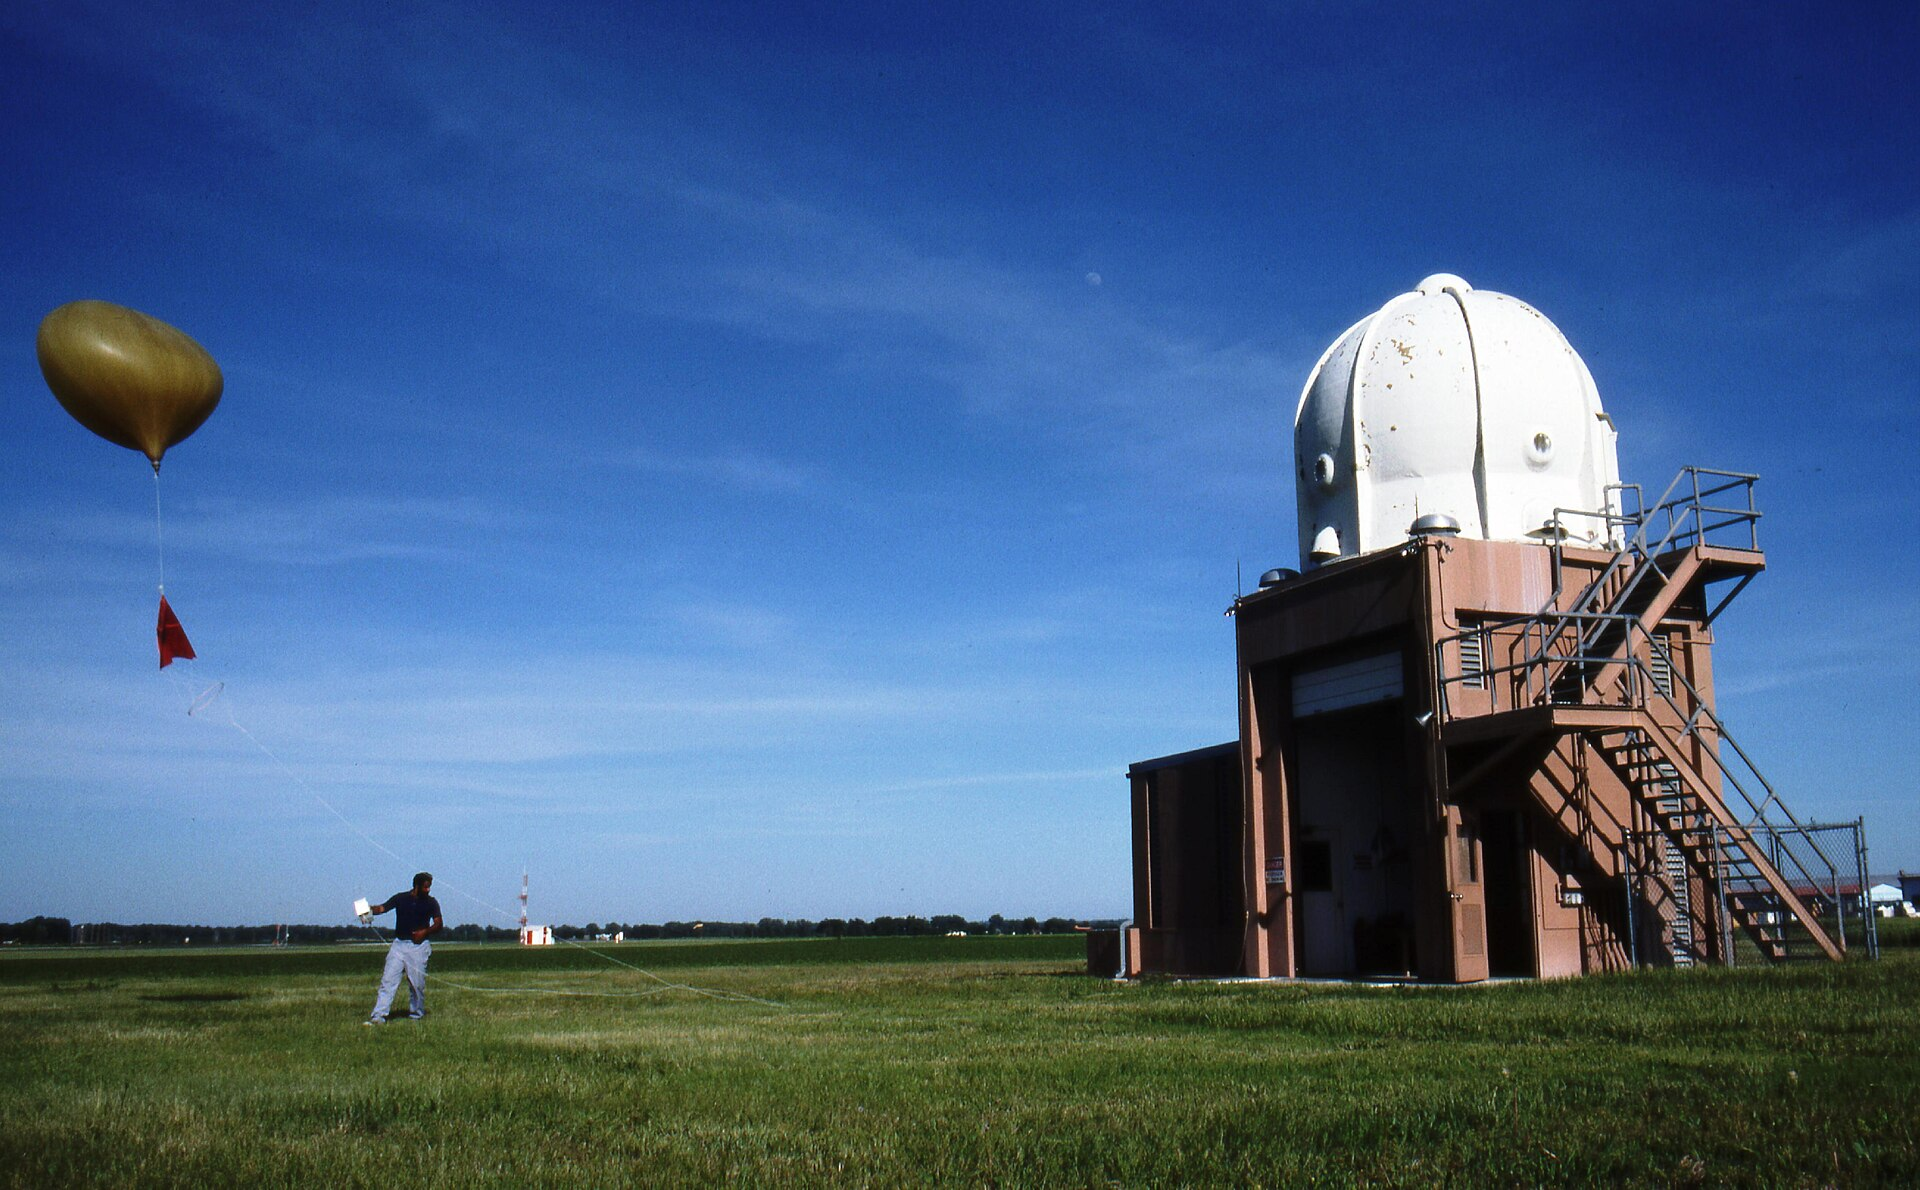
\includegraphics[width=0.78\linewidth]{images/book1/g8-radiosonde-launch.jpg}

{\small Een weerballon wordt opgelaten in Topeka, Kansas (Verenigde
Staten): de parachute (rood) en de radiosonde hangen onder de ballon. Foto
van Stephen Corfidi, NOAA/National Weather Service (publiek domein, via
Wikimedia Commons).}
% ledger: commons:radiosonde-launch
\label{fig:g8:the-atmosphere:launch}
\end{omfigure}

Waarom zwelt de ballon op terwijl hij stijgt? Wat meet de radiosonde op weg
naar boven, en waarom blijft de temperatuur niet gewoon \omterm{def:g1:landscapes-around-us:landform}{dalen}? Waar houdt de
lucht op?

\begin{recall}
De \emph{atmosfeer} is de laag lucht rond de Aarde. Lucht drukt op alles
wat ze raakt: dat is de \emph{luchtdruk}, gemeten met een barometer (de
natuurkundeboeken). Weerdiensten geven hem in hectopascal (hPa); op
\omterm{def:g4:world-physical-map:altitude}{zeeniveau} is hij ongeveer \qty{1013}{hPa}. Droge lucht bestaat voor
ongeveer 78~\% uit stikstof en 21~\% uit zuurstof, met een beetje argon,
koolstofdioxide en andere gassen (de scheikundeboeken). \omterm{def:g4:clouds-rain-snow:cloud}{Wolken} bestaan uit
piepkleine waterdruppeltjes of ijskristallen (\cref{ch:g4:clouds-rain-snow}).
\end{recall}
% ledger: air:N2, air:O2, ussa76:sea-level

\section{Een dun omhulsel}

Gezien vanuit het Internationale Ruimtestation is de atmosfeer een dunne
gloeiende lijn langs de rand van de Aarde. Het grootste deel van de lucht,
en bijna alle \omterm{def:g4:clouds-rain-snow:cloud}{wolken}, bevinden zich in de onderste paar kilometers.
% ledger: commons:iss-sunset

\begin{omfigure}
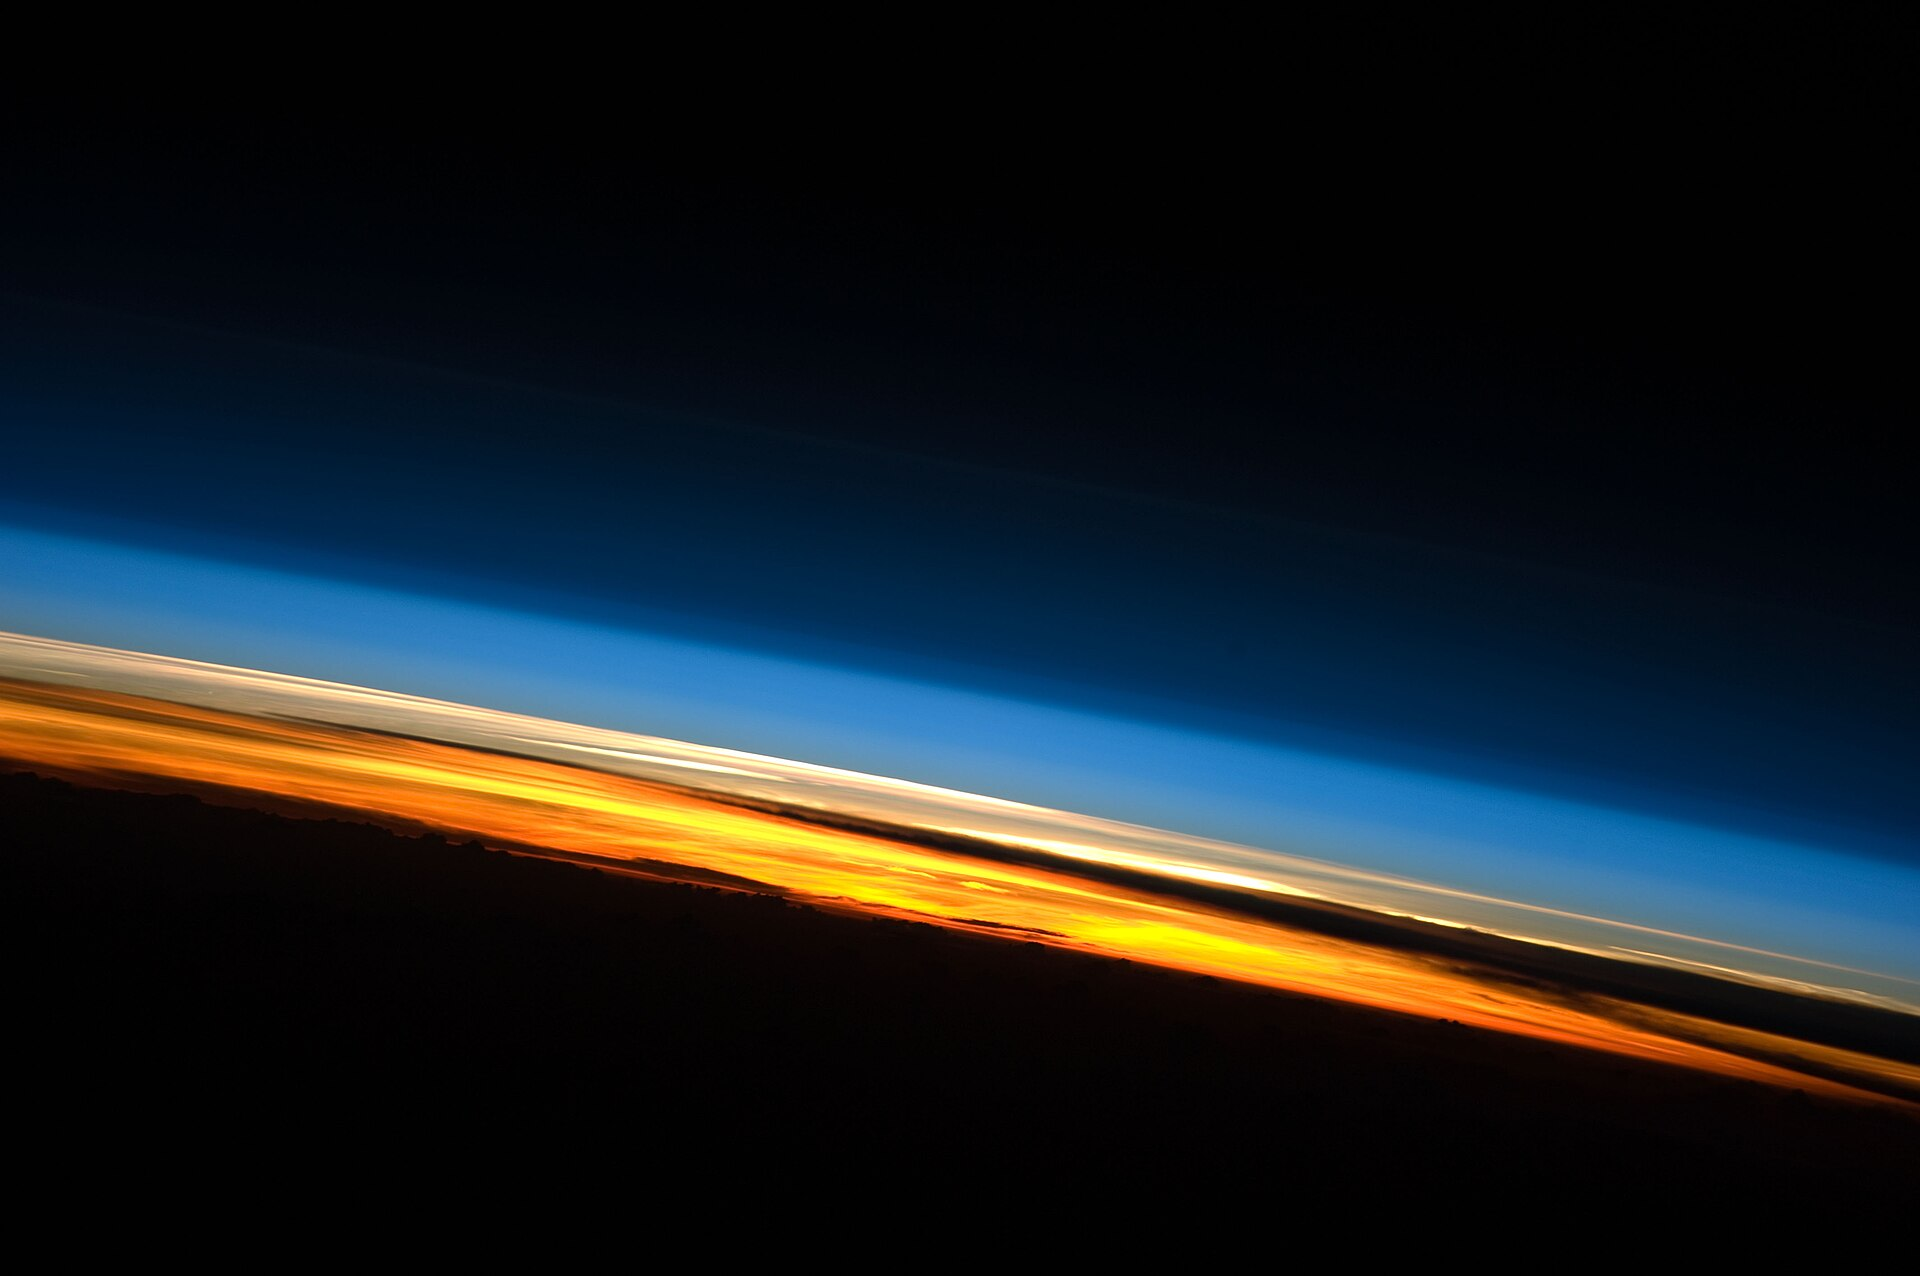
\includegraphics[width=0.78\linewidth]{images/book1/g8-iss-limb.jpg}

{\small De rand van de Aarde bij zonsondergang, gefotografeerd vanuit het
Internationale Ruimtestation boven de Indische \omterm{def:g2:water-on-earth:ocean}{Oceaan} op 14~juni 2010. De
oranje en gele band is de onderste laag van de atmosfeer, met haar donkere
\omterm{def:g4:clouds-rain-snow:cloud}{wolken}; daarboven komen lichtere en dan blauwe lagen, die overgaan in het
zwart van de ruimte. Foto van NASA, ISS Expedition~23 (publiek domein, via
Wikimedia Commons).}
% ledger: commons:iss-sunset
\label{fig:g8:the-atmosphere:limb}
\end{omfigure}

De atmosfeer heeft geen scherpe bovengrens: de lucht wordt met de hoogte
steeds ijler. Volgens afspraak begint de ruimte op ongeveer \qty{100}{km}.
Vergeleken met de straal van de Aarde, \qty{6371}{km}, is dat heel weinig:
$100 \div
6371 \approx 0.016$, minder dan 2~\% van de straal. Op een \omterm{def:g3:continents-and-oceans:globe}{globe} van
\qty{30}{cm} doorsnee zou de hele atmosfeer een laagje van ongeveer
\qty{2}{mm} dik zijn.
% ledger: ucar:layers, earth:Rmean

\begin{omfigure}
\begin{tikzpicture}[font=\footnotesize]
  % 1 cm = 100 km: the Earth's surface is a circle of radius 63.71 cm
  \def\R{63.71}
  \useasboundingbox (-6.9,-1.6) rectangle (6.9,1.0);
  \fill[blue!8] (0,-\R) ++(85:\R+1) arc (85:95:\R+1) -- ($(0,-\R)+(95:\R)$) arc (95:85:\R) -- cycle;
  \fill[omLithAlluv!70] (0,-\R) ++(85:\R) arc (85:95:\R) -- ++(0,-0.6) -- ($(0,-\R)+(85:\R)+(0,-0.6)$) -- cycle;
  \draw[black, line width=0.6pt] (0,-\R) ++(85:\R) arc (85:95:\R);
  \foreach \h/\c in {0.1102/omThm, 0.4938/omMeth, 0.86/omDef} \draw[\c, line width=0.5pt] (0,-\R) ++(85:\R+\h) arc (85:95:\R+\h);
  \draw[black!60, dashed] (0,-\R) ++(85:\R+1) arc (85:95:\R+1);
  \node[anchor=west, omThm] at (5.65,-0.14) {\qty{11}{km}};
  \node[anchor=west, omMeth] at (5.65,0.25) {\qty{49}{km}};
  \node[anchor=west, omDef] at (5.65,0.62) {\qty{86}{km}};
  \node[anchor=east, black!70] at (-5.65,0.75) {\qty{100}{km}};
  \node[anchor=north] at (0,-0.15) {het aardoppervlak};
  \draw[|-|] (-5,-1.05) -- node[below] {\qty{1000}{km}} (5,-1.05);
\end{tikzpicture}

{\small Een plak van de Aarde en haar atmosfeer op schaal getekend
(\qty{1}{cm} voor \qty{100}{km}), tot \qty{100}{km}, de rand van de ruimte
(gestippeld). De gekleurde lijnen zijn de grenzen van de lagen die verderop
in dit hoofdstuk aan bod komen; de onderste laag, waar al het \omterm{def:g1:watching-the-weather:weather}{weer} zich
afspeelt, is amper een millimeter dik.}
% ledger: earth:Rmean, ucar:layers (limits: figdata/grade-8/standard_atmosphere.py main table)
\label{fig:g8:the-atmosphere:to-scale}
\end{omfigure}

\section{De druk neemt af met de hoogte}

De lucht onderin de atmosfeer draagt het gewicht van alle lucht erboven. Hoe
hoger je klimt, hoe minder lucht er boven je overblijft, en hoe lager de
druk. In het standaardmodel van de atmosfeer dat meteorologen en ingenieurs
gebruiken, is de druk op \omterm{def:g4:world-physical-map:altitude}{zeeniveau} \qty{1013}{hPa}, op ongeveer
\qty{5.5}{km} de helft daarvan, en op ongeveer \qty{10.3}{km} een kwart.
% ledger: ussa76:sea-level, ussa76:layers (figdata/grade-8/standard_atmosphere.py main table: half_km 5.48, quarter_km 10.29)

Omdat de druk het gewicht van de lucht erboven meet, is het niveau van de
halve druk ook de hoogte waaronder de helft van alle lucht ligt: de helft
van de atmosfeer is samengeperst in haar onderste \qty{5.5}{km}. Onder
\qty{11}{km} ligt ongeveer 78~\% van de lucht, onder \qty{30}{km} ongeveer
99~\%.
% ledger: (computed: figdata/grade-8/standard_atmosphere.py, share_below_11km 77.7, share_below_30km 98.82)

\begin{omfigure}
\begin{minipage}[t]{0.49\linewidth}\centering
\begin{tikzpicture}
\begin{axis}[width=6.6cm, height=7.6cm, xmin=0, xmax=1100, ymin=0, ymax=30,
  xlabel={druk (hPa)}, ylabel={hoogte (km)},
  tick label style={font=\scriptsize}, label style={font=\small},
  xtick={0,250,500,750,1000}, ytick={0,5,10,15,20,25,30}]
  \addplot[dashed, black!60] table {figdata/out/grade-8-standard_atmosphere-guides.dat};
  \addplot[omDef, line width=1.1pt] table[x=p_hPa, y=z_km] {figdata/out/grade-8-standard_atmosphere-pressure.dat};
  \addplot[only marks, mark=*, mark size=1.8pt, omThm, nodes near coords, point meta=explicit symbolic,
    every node near coord/.style={anchor=south west, font=\scriptsize, text=black}]
    table[row sep=\\, x=p_hPa, y=z_km, meta=label] {z_km p_hPa label\\ 5.48 506.6 {de helft}\\ 10.29 253.3 {een kwart}\\ };
\end{axis}
\end{tikzpicture}

{\small Druk tegen hoogte. De druk is op ongeveer \qty{5.5}{km} de helft
van zijn waarde op \omterm{def:g4:world-physical-map:altitude}{zeeniveau}, op ongeveer \qty{10.3}{km} een kwart.}
\end{minipage}\hfill
\begin{minipage}[t]{0.49\linewidth}\centering
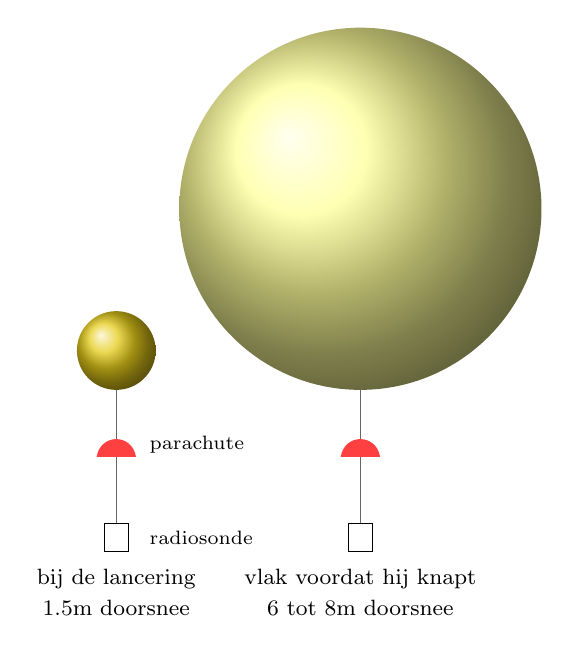
\begin{tikzpicture}[font=\footnotesize]
  % at launch: 1.5 m; at burst: about 7 m (drawn 1 cm for 1.5 m)
  \draw[black!60] (0,0.9) -- (0,2.6);
  \shade[ball color=yellow!60!brown] (0,3.1) circle (0.5);
  \fill[red!75] (-0.25,1.75) .. controls (-0.2,2.05) and (0.2,2.05) .. (0.25,1.75) -- cycle;
  \fill[white, draw=black] (-0.15,0.55) rectangle (0.15,0.9);
  \node[anchor=north] at (0,0.45) {bij de lancering};
  \node[anchor=north] at (0,0.05) {\qty{1.5}{m} doorsnee};
  \begin{scope}[xshift=3.1cm]
    \draw[black!60] (0,0.9) -- (0,2.6);
    \shade[ball color=yellow!40!white] (0,4.9) circle (2.3);
    \fill[red!75] (-0.25,1.75) .. controls (-0.2,2.05) and (0.2,2.05) .. (0.25,1.75) -- cycle;
    \fill[white, draw=black] (-0.15,0.55) rectangle (0.15,0.9);
    \node[anchor=north] at (0,0.45) {vlak voordat hij knapt};
    \node[anchor=north] at (0,0.05) {6 tot \qty{8}{m} doorsnee};
  \end{scope}
  \node[anchor=west, font=\scriptsize] at (0.3,1.9) {parachute};
  \node[anchor=west, font=\scriptsize] at (0.3,0.72) {radiosonde};
\end{tikzpicture}

{\small De ballon zwelt op terwijl hij stijgt, omdat de lucht eromheen
steeds minder hard drukt (ballonnen en parachutes onderling op schaal, het
touw ingekort).}
% ledger: nws:radiosonde
\end{minipage}
% ledger: ussa76:sea-level, ussa76:layers (figdata/grade-8/standard_atmosphere.py parts pressure, levels, guides)
\label{fig:g8:the-atmosphere:pressure}
\end{omfigure}

Hoger blijft de druk \omterm{def:g1:landscapes-around-us:landform}{dalen}, telkens met ongeveer de helft na een paar
kilometer, zodat hij al snel heel klein wordt. Machten van tien zijn de
beste manier om hem te schrijven. Op \qty{30}{km} is de druk ongeveer
\qty{12}{hPa}, ruwweg $10^{-2}$ van zijn waarde op \omterm{def:g4:world-physical-map:altitude}{zeeniveau} (een
honderdste); op \qty{50}{km} ongeveer \qty{0.8}{hPa}, ruwweg $10^{-3}$; op
\qty{80}{km} ongeveer \qty{0.01}{hPa}, ruwweg $10^{-5}$ van de druk op
\omterm{def:g4:world-physical-map:altitude}{zeeniveau}.
% ledger: ussa76:layers (figdata/grade-8/standard_atmosphere.py main table: p_30km 11.97, p_50km 0.798, p_80km 0.0105 hPa)

\begin{omfigure}
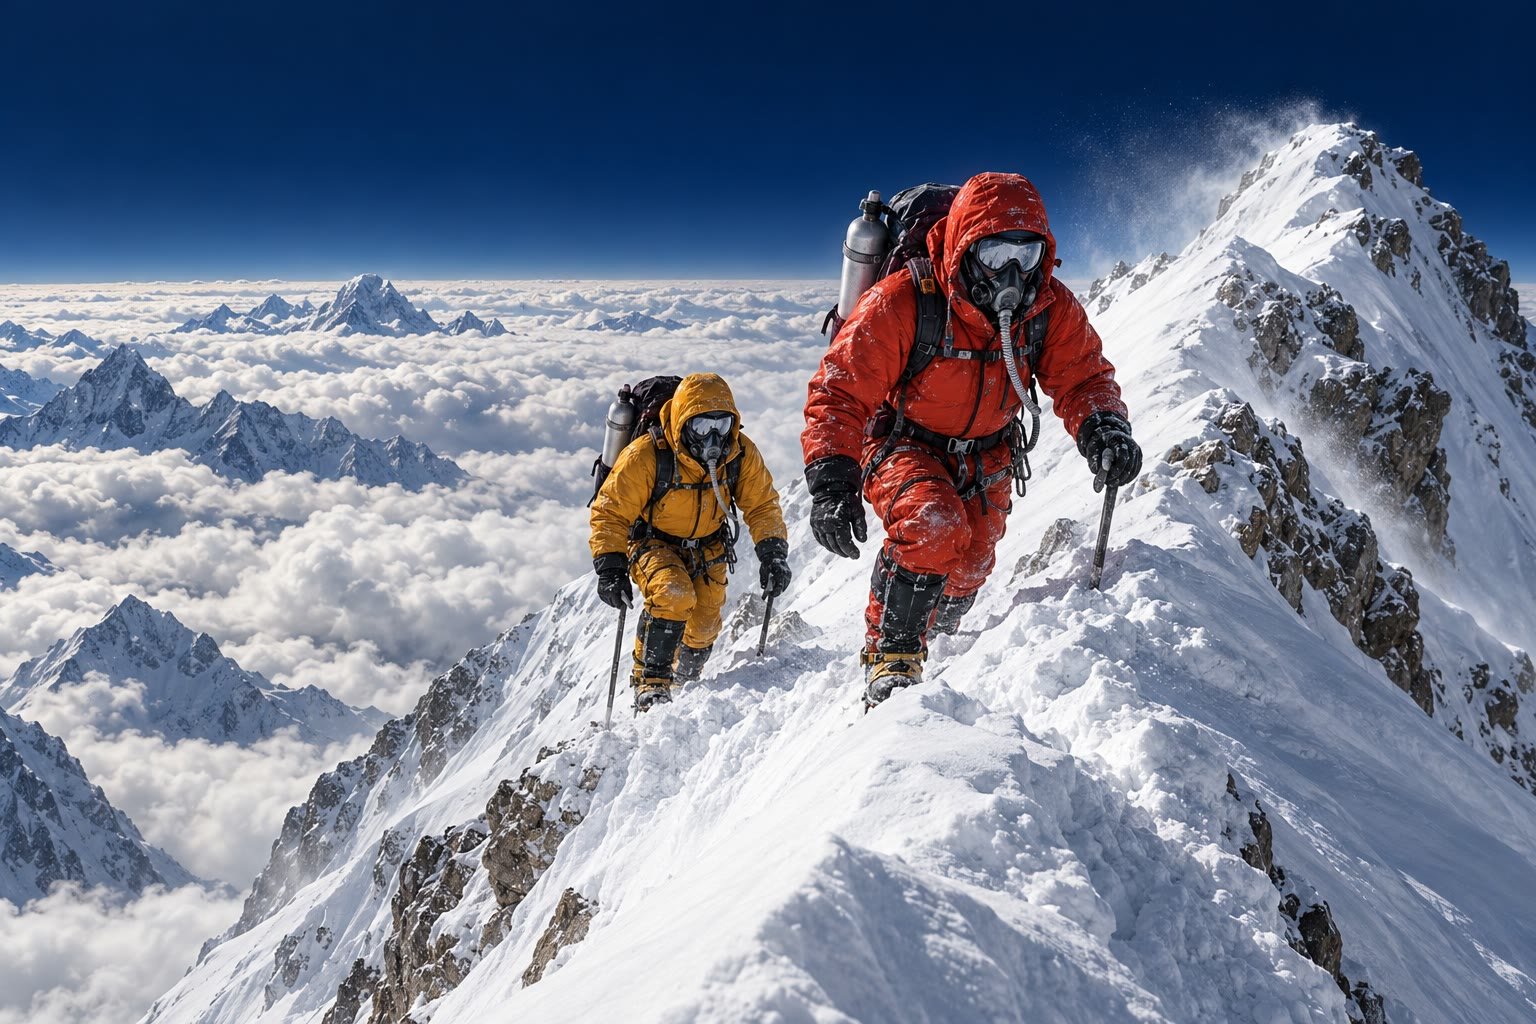
\includegraphics[width=0.5\linewidth]{images/book1/ai/g8-climbers.jpg}

{\small Klimmers op een heel hoge \omterm{def:g1:landscapes-around-us:landform}{berg} dragen zuurstofflessen mee. Op
\qty{9}{km} is de druk minder dan een derde van zijn waarde op \omterm{def:g4:world-physical-map:altitude}{zeeniveau}:
de lucht bevat nog steeds 21~\% zuurstof, maar elke ademteug neemt er veel
minder van op (door AI gegenereerde illustratie van een algemene scène).}
% ledger: air:O2 (figdata/grade-8/standard_atmosphere.py: pressure at 9 km 308 hPa, 30 % of sea level)
\label{fig:g8:the-atmosphere:climbers}
\end{omfigure}

\section{Temperatuur en de lagen}

Iedereen die een \omterm{def:g1:landscapes-around-us:landform}{berg} heeft beklommen, weet dat de lucht met de hoogte
kouder wordt. De radiosondes laten zien dat dit alleen in het onderste deel
van de atmosfeer klopt. Hoger stopt de temperatuur met \omterm{def:g1:landscapes-around-us:landform}{dalen}, dan stijgt
ze, dan daalt ze weer, en dan stijgt ze nog eens. Deze veranderingen
verdelen de atmosfeer in lagen.
% ledger: ucar:layers, ussa76:layers

\begin{omfigure}
\begin{tikzpicture}
\begin{axis}[width=10cm, height=9cm, xmin=-100, xmax=30, ymin=0, ymax=100,
  xlabel={temperatuur ($^\circ$C)}, ylabel={hoogte (km)},
  tick label style={font=\scriptsize}, label style={font=\small},
  xtick={-100,-80,-60,-40,-20,0,20}, ytick={0,10,20,30,40,50,60,70,80,90,100}, axis on top]
  \addplot[fill=omSea!55, draw=none] table {figdata/out/grade-8-standard_atmosphere-band-troposphere.dat};
  \addplot[fill=omMeth!12, draw=none] table {figdata/out/grade-8-standard_atmosphere-band-stratosphere.dat};
  \addplot[fill=omSea!35, draw=none] table {figdata/out/grade-8-standard_atmosphere-band-mesosphere.dat};
  \addplot[fill=omThm!10, draw=none] table {figdata/out/grade-8-standard_atmosphere-band-thermosphere.dat};
  \addplot[omThm, line width=1.2pt] table[x=T_C, y=z_km] {figdata/out/grade-8-standard_atmosphere-temp.dat};
  \addplot[draw=none, nodes near coords, point meta=explicit symbolic,
    every node near coord/.style={anchor=west, font=\small\bfseries, text=black!75}]
    table[row sep=\\, x=lx_C, y=mid_km, meta=name] {name base_km top_km mid_km lx_C\\ troposfeer 0 11.02 5.51 -97\\ stratosfeer 11.02 49.38 30.2 -97\\ mesosfeer 49.38 86 67.69 -97\\ thermosfeer 86 100 93 -60\\ };
  \draw[black!50, dashed] (axis cs:-100,11.02) -- (axis cs:30,11.02);
  \draw[black!50, dashed] (axis cs:-100,49.38) -- (axis cs:30,49.38);
  \draw[black!50, dashed] (axis cs:-100,86) -- (axis cs:30,86);
  \node[anchor=south east, font=\scriptsize] at (axis cs:17,11.02) {tropopauze};
  \node[anchor=south east, font=\scriptsize] at (axis cs:29,49.38) {stratopauze};
  \node[anchor=south east, font=\scriptsize] at (axis cs:29,86) {mesopauze};
  \fill[omMeth!45] (axis cs:19,16) rectangle (axis cs:23,48);
  \node[anchor=east, font=\scriptsize, align=right] at (axis cs:18,30) {ozon-\\laag};
\end{axis}
\end{tikzpicture}

{\small De temperatuur van de lucht tegen de hoogte, van de grond tot
\qty{100}{km}, in de standaardatmosfeer (een gemiddelde voor de gematigde
breedten). De vier lagen zijn ingekleurd; de groene balk geeft de hoogte van
de \omterm{def:g8:the-atmosphere:ozone-layer}{ozonlaag} aan.}
% ledger: ussa76:sea-level, ussa76:layers, ussa76:above-86, ucar:ozone (figdata/grade-8/standard_atmosphere.py parts temp, layers, band-*)
\label{fig:g8:the-atmosphere:temperature}
\end{omfigure}

\begin{definition}[De lagen van de atmosfeer]\label{def:g8:the-atmosphere:layers}
Van de grond af naar boven is de atmosfeer verdeeld in vier lagen, naar de
manier waarop haar temperatuur met de hoogte verandert:
\begin{itemize}
  \item de \emph{troposfeer}\index{troposfeer}, waar de temperatuur met de
        hoogte daalt en waar bijna al het \omterm{def:g1:watching-the-weather:weather}{weer} zich afspeelt; haar
        bovengrens is de \emph{tropopauze}\index{tropopauze};
  \item de \emph{stratosfeer}\index{stratosfeer}, waar de temperatuur met
        de hoogte stijgt, tot ongeveer \qty{50}{km};
  \item de \emph{mesosfeer}\index{mesosfeer}, waar de temperatuur weer
        daalt, tot ongeveer \qty{85}{km};
  \item de \emph{thermosfeer}\index{thermosfeer}, waar de heel ijle lucht
        met de hoogte steeds heter wordt.
\end{itemize}
\end{definition}
% ledger: ucar:layers, ussa76:layers

De \omterm{def:g8:the-atmosphere:layers}{troposfeer} bevat ongeveer 99~\% van de waterdamp van de atmosfeer, dus
vormen bijna alle \omterm{def:g4:clouds-rain-snow:cloud}{wolken}, \omterm{def:g4:clouds-rain-snow:precipitation}{regen} en \omterm{def:g4:clouds-rain-snow:precipitation}{sneeuw} zich daarin. Haar lucht wordt
voortdurend omgewoeld. De bovenkant van de \omterm{def:g8:the-atmosphere:layers}{troposfeer} ligt niet overal op
dezelfde hoogte: de \omterm{def:g8:the-atmosphere:layers}{tropopauze} ligt het hoogst boven de \omterm{def:g3:continents-and-oceans:equator}{evenaar}, waar ze
\qty{20}{km} kan bereiken, en het laagst boven de \omterm{def:g3:continents-and-oceans:poles}{polen}, waar ze in de
winter tot \qty{7}{km} kan zakken. Ze ligt ook hoger in de zomer dan in de
winter. In de standaardatmosfeer, een gemiddelde voor de gematigde
breedten, ligt ze op \qty{11}{km}.
% ledger: ucar:layers, ucar:tropopause, ussa76:layers

\begin{definition}[Verticale temperatuurgradiënt]\label{def:g8:the-atmosphere:lapse-rate}
De \emph{verticale temperatuurgradiënt}\index{verticale temperatuurgradient@verticale temperatuurgradiënt}
is de snelheid waarmee de temperatuur van de lucht in de \omterm{def:g8:the-atmosphere:layers}{troposfeer} met de
hoogte daalt, in graden Celsius per kilometer. Hij verandert van dag tot
dag en van plaats tot plaats; de standaardatmosfeer gebruikt een
gemiddelde van \qty{6.5}{\degreeCelsius} per kilometer.
\end{definition}
% ledger: ussa76:layers

\begin{method}[Een temperatuurprofiel lezen]\label{met:g8:the-atmosphere:profile}
\begin{enumerate}
  \item Zoek de hoogte op de verticale as en ga horizontaal naar de
        kromme; lees de temperatuur eronder af.
  \item Waar de kromme naar boven toe naar links helt, koelt de lucht af
        met de hoogte; waar ze naar rechts helt, warmt de lucht op met de
        hoogte; waar ze verticaal staat, verandert de temperatuur niet.
  \item De grenzen tussen de lagen liggen waar de kromme van richting
        verandert.
\end{enumerate}
\end{method}

\begin{example}[Een lijnvliegtuig op kruishoogte]\label{ex:g8:the-atmosphere:airliner}
Een lijnvliegtuig vliegt op \qty{11}{km}, bij de \omterm{def:g8:the-atmosphere:layers}{tropopauze}. Op het profiel
is de temperatuur daar ongeveer \qty{-56}{\degreeCelsius}. Met de
temperatuurgradiënt: vanaf \qty{15}{\degreeCelsius} op \omterm{def:g4:world-physical-map:altitude}{zeeniveau} koelt de
lucht $6.5 \times 11 = 71.5$ graden af, wat $15 - 71.5 =
\qty{-56.5}{\degreeCelsius}$ geeft. Op de drukkromme is de druk ongeveer
\qty{227}{hPa}, minder dan een kwart van de druk op de grond: de cabine moet
onder druk worden gezet.
% ledger: ussa76:sea-level, ussa76:layers (figdata/grade-8/standard_atmosphere.py: T at 11 km -56.4 degC, p 227 hPa)
\end{example}

Boven de \omterm{def:g8:the-atmosphere:layers}{tropopauze}, in de \omterm{def:g8:the-atmosphere:layers}{stratosfeer}, vinden lijnvliegtuigen een rustiger
vlucht: de lucht daar wordt met de hoogte warmer, dus wordt ze niet van
onderaf omgewoeld. In de \omterm{def:g8:the-atmosphere:layers}{mesosfeer} verbranden de meeste meteoren, en aan
haar bovenkant, rond \qty{86}{km}, bevindt zich de koudste lucht van de hele
atmosfeer, ongeveer \qty{-86}{\degreeCelsius}. In de \omterm{def:g8:the-atmosphere:layers}{thermosfeer} verhitten
de röntgenstraling en het ultraviolette licht van de Zon de heel ijle lucht
tot honderden, soms duizenden graden; toch is er zo weinig lucht dat ze
niet warm zou aanvoelen. Veel satellieten draaien daar om de Aarde.
% ledger: ucar:layers, ussa76:above-86

\section{De ozonlaag}

De \omterm{def:g8:the-atmosphere:layers}{stratosfeer} wordt met de hoogte warmer omdat ze een deel van het
zonlicht absorbeert. Het gas dat het meeste daarvan doet, is ozon, een vorm
van zuurstof (de scheikunde ervan staat in de scheikundeboeken).

\begin{definition}[Ozonlaag]\label{def:g8:the-atmosphere:ozone-layer}
De \emph{ozonlaag}\index{ozonlaag} is het deel van de \omterm{def:g8:the-atmosphere:layers}{stratosfeer}, tussen
ongeveer \qty{16}{km} en \qty{48}{km}, waar ongeveer 90~\% van het ozon van
de atmosfeer zit. Ze absorbeert het grootste deel van het schadelijke
ultraviolette licht van de Zon.
\end{definition}
% ledger: ucar:ozone

Zelfs in de \omterm{def:g8:the-atmosphere:ozone-layer}{ozonlaag} is ozon zeldzaam: maar 1 tot 10 moleculen op een
miljoen. Toch houdt het samen met zuurstof tussen 95~\% en 99.9~\% tegen
van het ultraviolette licht dat de Aarde bereikt, ook de schadelijkste
soorten. De energie die het absorbeert, wordt omgezet in warmte; daarom
stijgt de temperatuur door de \omterm{def:g8:the-atmosphere:layers}{stratosfeer} heen. Zonder de \omterm{def:g8:the-atmosphere:ozone-layer}{ozonlaag} zou het
ultraviolette licht dat de grond bereikt levende wezens schaden.
% ledger: ucar:ozone

\begin{inthefield}[De weerballonnen volgen]
Weerdiensten publiceren de metingen van hun radiosondes, vaak als een
diagram van de temperatuur tegen de hoogte voor elke lancering. Zoek samen
met een volwassene de peilingen op van het station dat het dichtst bij je
ligt, gedaan om 00.00 of 12.00 uur UTC. Zoek de hoogte waar de temperatuur
stopt met \omterm{def:g1:landscapes-around-us:landform}{dalen}: dat is de \omterm{def:g8:the-atmosphere:layers}{tropopauze} op die dag. Vergelijk een peiling in
de winter met een in de zomer.
\end{inthefield}
% ledger: nws:radiosonde, ucar:tropopause

\section{Oefeningen}

\begin{exercise}[$\star$]\label{exo:g8:the-atmosphere:1}
Koppel elke laag aan haar beschrijving: \omterm{def:g8:the-atmosphere:layers}{troposfeer}; \omterm{def:g8:the-atmosphere:layers}{stratosfeer};
\omterm{def:g8:the-atmosphere:layers}{mesosfeer}; \omterm{def:g8:the-atmosphere:layers}{thermosfeer}. (a) De temperatuur stijgt met de hoogte en de
\omterm{def:g8:the-atmosphere:ozone-layer}{ozonlaag} bevindt zich daar. (b) Bijna al het \omterm{def:g1:watching-the-weather:weather}{weer} speelt zich daar af.
(c) De koudste lucht van de atmosfeer bevindt zich aan de bovenkant ervan.
(d) De heel ijle lucht wordt tot honderden graden verhit; veel satellieten
draaien daar.
\end{exercise}

\begin{exercise}[$\star$]\label{exo:g8:the-atmosphere:2}
Gebruik het temperatuurprofiel van de standaardatmosfeer. (a) Wat is de
temperatuur op \omterm{def:g4:world-physical-map:altitude}{zeeniveau}? (b) Op \qty{11}{km}? (c) Op \qty{50}{km}?
(d) Op \qty{86}{km}? (e) Tussen welke hoogten verandert de temperatuur
niet?
\end{exercise}

\begin{exercise}[$\star$]\label{exo:g8:the-atmosphere:3}
Waar of niet waar? Verbeter de onware zinnen. (a) De temperatuur van de
lucht daalt altijd met de hoogte. (b) De helft van alle lucht ligt onder
ongeveer \qty{5.5}{km}. (c) De \omterm{def:g8:the-atmosphere:ozone-layer}{ozonlaag} bevindt zich in de \omterm{def:g8:the-atmosphere:layers}{troposfeer}.
(d) De \omterm{def:g8:the-atmosphere:layers}{tropopauze} ligt boven de \omterm{def:g3:continents-and-oceans:equator}{evenaar} hoger dan boven de \omterm{def:g3:continents-and-oceans:poles}{polen}.
\end{exercise}

\begin{exercise}[$\star$]\label{exo:g8:the-atmosphere:4}
In welke laag bevindt elk van deze zich? (a) Een regenwolk. (b) Een
lijnvliegtuig op \qty{12}{km}. (c) Een weerballon vlak voordat hij knapt,
op \qty{32}{km}. (d) Een meteoor die op \qty{75}{km} verbrandt.
\end{exercise}

\begin{exercise}[$\star\star$]\label{exo:g8:the-atmosphere:5}
Op een zomerdag is het op \omterm{def:g4:world-physical-map:altitude}{zeeniveau} \qty{20}{\degreeCelsius}. Stel dat de
lucht \qty{6.5}{\degreeCelsius} per kilometer afkoelt. (a) Wat is de
temperatuur op \qty{2}{km}? (b) Op \qty{3}{km}? (c) Op ongeveer welke
hoogte bereikt de lucht \qty{0}{\degreeCelsius}? Rond af op één decimaal.
\end{exercise}

\begin{exercise}[$\star\star$]\label{exo:g8:the-atmosphere:6}
Een berghut staat op \qty{3000}{m}. Een wandelaar vertrekt uit een dorp op
\qty{500}{m}, waar het \qty{18}{\degreeCelsius} is. Met een
temperatuurgradiënt van \qty{6.5}{\degreeCelsius} per kilometer: (a) Hoeveel
kilometer klimt de wandelaar? (b) Hoeveel graden koelt de lucht af?
(c) Welke temperatuur kan de wandelaar bij de hut verwachten?
\end{exercise}

\begin{exercise}[$\star\star$]\label{exo:g8:the-atmosphere:7}
Stel dat de druk elke \qty{5.5}{km} halveert, te beginnen met
\qty{1000}{hPa} op \omterm{def:g4:world-physical-map:altitude}{zeeniveau}. (a) Wat is de druk op \qty{5.5}{km}? Op
\qty{11}{km}? Op \qty{16.5}{km}? (b) De standaardatmosfeer geeft op deze
drie hoogten ongeveer \qty{506}{hPa}, \qty{227}{hPa} en \qty{96}{hPa} (bij
\qty{1013}{hPa} op \omterm{def:g4:world-physical-map:altitude}{zeeniveau}). Is de halveringsregel goed dicht bij de
grond? En hoger?
\end{exercise}

\begin{exercise}[$\star\star$]\label{exo:g8:the-atmosphere:8}
Op \omterm{def:g4:world-physical-map:altitude}{zeeniveau} is de druk ongeveer \qty{1000}{hPa}, dat is $10^3$~hPa. (a) Op
\qty{30}{km} is hij ongeveer \qty{10}{hPa}. Schrijf dit als een macht van
tien, en zeg hoeveel keer kleiner hij is dan op \omterm{def:g4:world-physical-map:altitude}{zeeniveau}. (b) Op
\qty{80}{km} is hij ongeveer \qty{0.01}{hPa}. Schrijf dit als een macht van
tien. (c) Hoeveel keer kleiner dan op \omterm{def:g4:world-physical-map:altitude}{zeeniveau} is hij?
\end{exercise}

\begin{exercise}[$\star\star$]\label{exo:g8:the-atmosphere:9}
Een weerballon is bij de lancering \qty{1.5}{m} in doorsnee en
\qty{6}{m} als hij knapt. (a) Hoeveel keer breder is hij als hij knapt?
(b) Leg uit waarom hij opzwelt terwijl hij stijgt. (c) Waarom hangen
weerdiensten er een parachute onder?
\end{exercise}

\begin{exercise}[$\star\star$]\label{exo:g8:the-atmosphere:10}
De \omterm{def:g8:the-atmosphere:layers}{tropopauze} kan boven de \omterm{def:g3:continents-and-oceans:equator}{evenaar} \qty{20}{km} bereiken en boven de \omterm{def:g3:continents-and-oceans:poles}{polen}
in de winter tot \qty{7}{km} zakken. (a) Hoeveel keer dikker is de
\omterm{def:g8:the-atmosphere:layers}{troposfeer} boven de \omterm{def:g3:continents-and-oceans:equator}{evenaar} in dit geval? Rond af op één decimaal. (b) Op
het standaardprofiel ligt de \omterm{def:g8:the-atmosphere:layers}{tropopauze} op \qty{11}{km}. Ligt de
standaardatmosfeer dichter bij die van de \omterm{def:g3:continents-and-oceans:equator}{evenaar} of bij die van de \omterm{def:g3:continents-and-oceans:poles}{polen}?
(c) Een piloot vliegt van een poolgebied naar de \omterm{def:g3:continents-and-oceans:equator}{evenaar} op een vaste
hoogte van \qty{10}{km}. Bevindt het vliegtuig zich aan het begin (in de
winter) in de \omterm{def:g8:the-atmosphere:layers}{troposfeer} of in de \omterm{def:g8:the-atmosphere:layers}{stratosfeer}? En aan het eind?
\end{exercise}

\begin{exercise}[$\star\star\star$]\label{exo:g8:the-atmosphere:11}
Het deel van alle lucht dat onder een bepaalde hoogte ligt, is $1 - p \div
p_0$, waarbij $p$ de druk op die hoogte is en $p_0 =
\qty{1013}{hPa}$ de druk op \omterm{def:g4:world-physical-map:altitude}{zeeniveau}. (a) Op \qty{5.5}{km} is $p
\approx \qty{506}{hPa}$: welk deel van de lucht ligt eronder? (b) Op
\qty{11}{km} is $p \approx \qty{227}{hPa}$. (c) Op \qty{30}{km} is $p \approx
\qty{12}{hPa}$. Geef de antwoorden in procenten, in hele getallen. (d) Welk
deel van de lucht ligt boven \qty{30}{km}?
\end{exercise}

\begin{exercise}[$\star\star\star$]\label{exo:g8:the-atmosphere:12}
Een schoolglobe is \qty{30}{cm} in doorsnee, dus zijn straal, \qty{15}{cm},
staat voor de straal van de Aarde, \qty{6371}{km}. (a) Voor hoeveel
kilometer staat \qty{1}{cm} op de \omterm{def:g3:continents-and-oceans:globe}{globe}? Rond af op een hele kilometer.
(b) Hoe dik, in millimeter, zou de atmosfeer tot \qty{100}{km} op deze
\omterm{def:g3:continents-and-oceans:globe}{globe} zijn? (c) En de \omterm{def:g8:the-atmosphere:layers}{troposfeer}, die \qty{11}{km} dik is? (d) Een vel
papier is ongeveer \qty{0.1}{mm} dik. Hoeveel vellen zouden de \omterm{def:g8:the-atmosphere:layers}{troposfeer}
van de \omterm{def:g3:continents-and-oceans:globe}{globe} vormen?
\end{exercise}

\section{Probleem: Een weerballon volgen}

\begin{problem}[{Weekendprobleem --- een weerballon stijgt door de
atmosfeer; zijn temperaturen tonen de lagen, en zijn drukken tonen waar nog
een kwart van de druk op zeeniveau over is}]
\label{pb:g8:the-atmosphere:1}
% ledger: nws:radiosonde; the table is the standard atmosphere, figdata/grade-8/standard_atmosphere.py part sonde
Een radiosonde wordt opgelaten vanaf een station op \omterm{def:g4:world-physical-map:altitude}{zeeniveau}. De ballon
stijgt met ongeveer \qty{300}{m} per minuut. De tabel geeft de druk en de
temperatuur die de sonde meet (de waarden van de standaardatmosfeer,
afgerond).

\begin{center}\small
\begin{tabular}{|l|*{8}{c|}}
\hline
hoogte (km) & 0 & 2 & 4 & 6 & 8 & 10 & 12 & 14 \\
\hline
druk (hPa) & 1013 & 795 & 617 & 472 & 357 & 265 & 194 & 142 \\
\hline
temperatuur ($^\circ$C) & 15 & 2 & $-11$ & $-24$ & $-37$ & $-50$ & $-56$ & $-56$ \\
\hline
\hline
hoogte (km) & 16 & 18 & 20 & 22 & 24 & 26 & 28 & 30 \\
\hline
druk (hPa) & 104 & 76 & 55 & 40 & 30 & 22 & 16 & 12 \\
\hline
temperatuur ($^\circ$C) & $-56$ & $-56$ & $-56$ & $-55$ & $-53$ & $-51$ & $-49$ & $-47$ \\
\hline
\end{tabular}
\end{center}

\noindent\textbf{Deel I --- De klim.}\par\nopagebreak
\begin{enumerate}[beginpenalty=10000]
  \item Hoeveel meter stijgt de ballon in 10 minuten?
  \item Hoe lang doet hij erover om \qty{6}{km} te bereiken? En
        \qty{30}{km}?
  \item De ballon knapt op \qty{30}{km}. Hoe lang heeft de vlucht geduurd,
        in uren en minuten?
  \item Noem de laag waarin de ballon zich op \qty{8}{km} bevindt, en de laag
        waarin hij zich bevindt als hij knapt.
\end{enumerate}

\noindent\textbf{Deel II --- De temperatuur.}\par\nopagebreak
\begin{enumerate}[resume, beginpenalty=10000]
  \item Hoeveel graden daalt de temperatuur tussen de grond en
        \qty{10}{km}?
  \item Wat is de temperatuurgradiënt in graden per kilometer in dit deel
        van de klim?
  \item Tussen welke hoogten blijft de temperatuur gelijk? Waar ligt de
        \omterm{def:g8:the-atmosphere:layers}{tropopauze}?
  \item Wat gebeurt er met de temperatuur boven \qty{20}{km}? Welk gas
        verklaart dat?
\end{enumerate}

\noindent\textbf{Deel III --- De druk.}\par\nopagebreak
\begin{enumerate}[resume, beginpenalty=10000]
  \item Wat is de helft van de druk op \omterm{def:g4:world-physical-map:altitude}{zeeniveau}? Tussen welke hoogten
        wordt die bereikt?
  \item Wat is een kwart van de druk op \omterm{def:g4:world-physical-map:altitude}{zeeniveau}? Rond af op een hele
        hectopascal.
  \item Tussen welke twee hoogten van de tabel wordt dit kwart bereikt?
  \item De druk daalt tussen \qty{10}{km} en \qty{12}{km} met
        \qty{71}{hPa}. Op ongeveer welke hoogte is de druk een kwart van
        zijn waarde op \omterm{def:g4:world-physical-map:altitude}{zeeniveau}, als je aanneemt dat hij gelijkmatig daalt?
        Rond af op één decimaal.
\end{enumerate}
\end{problem}
